um die grossen datenmengen die für ein robustes ML aus \ref{} benötigt werden liefern zu könne, muss die Messung die teure menschliche Arbeitszeit drastisch reduzieren. Die Vorstudien in \ref{} waren rund 9 h Arbeitszeit und haben rund 50 LWCTape und 6 LWCDenoth geliefert.


Ein grosser vorteil des Taps ist die feine örtliche auflösung von 20 x 20 mm. Um diese feine auflösung zu nutzen ist es spannend durch die Höhe der schneedecke die messungen durch zu führen.

in den kleinen Vorversuchen und den Funktionsmuster ist die Idee, dass ein Feldforscher einen Schneegraben gräbt und so Zugang an die unterschiedlichen Schichten hat.

Das Graben eines Schneegrabens ist aufwändig und sollte daher vermieden werden.

eine möglichkeit ist das der feldforscher mit einer bohrmaschine ein roch in den schnee macht. dann kann der feldforscher das messsystem in das loch herablassen, das kontinuierlich eine messung durchführt, während es herab gelassen wird.

Es ist auch möglich, dass das Messsystem über den Sommer an strategisch gewählten Orten aufgebaut wird und es dann eingeschneit wird. Hier ist die Schwierigkeit an genügend 'ungetesteten' guten Schnee dran zu kommen um eine feine zeitliche Auflösung zu ermöglichen.

Mit einer Vorstudie kann überprüft werden, wie sich Schnee verhält, wenn der Schnee ein zweites Mal getestet wird, und wie lange es braucht, bis sich der Schnee vom Test erholt hat. Wenn mit wenig Anpressdruck gearbeitet wird, kann ich mir vorstellen, dass sich der Schnee schnell erholt. Das würde die Umsetzung des Konzeptes massiv vereinfachen.

Ein weiteres Konzept ist, dass von einem Helikopter aus das Messsystem abgeworfen wird. durch die kinetische Energie schlägt das Messsystem dann durch die Schneedecke. In einer zweiten Phase wird dann das Tape an den Schnee angepresst und die Daten drahtlos an die Datenbank aus \ref{} eingespeist.

Um den Anpressdruck seitlich ausüben zu können, funktioniert die Schwerkraft nicht mehr. Elastomere sind bei tiefen Temperaturen schwer einzuschätzen. Ein Elektromotor ist möglich, aber etwas mühsam mit der Batterie. eine Blattfeder oder Kompressionsfeder sind vielversprechende Varianten.

Um eine hohe Anpassbarkeit des steifen Tapes an der schee zu ermoglichen, koann da sTape in kleinere Stücke geschnitten werden. So kann der elastische Träger des Tapes sich effektiv an den Schnee anpassen.


\begin{figure}
    \centering
    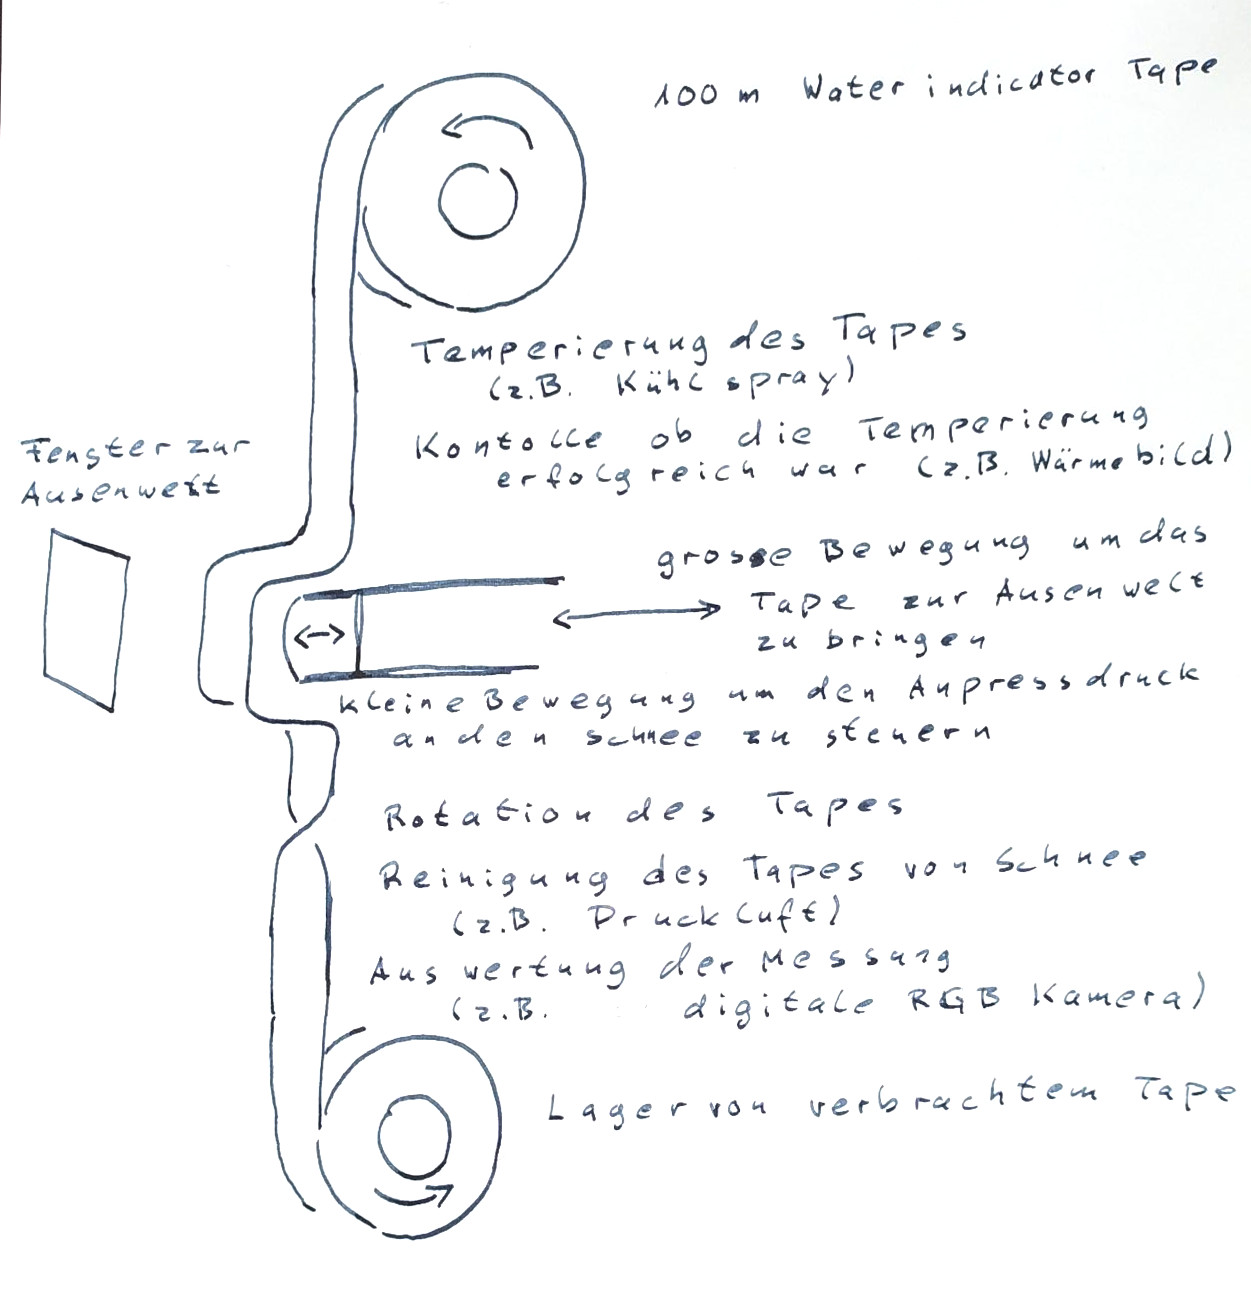
\includegraphics[width=0.8\textwidth]{Bilder/KonzeptAut.jpeg}
    \caption{Ablauf einer automatischen Messung}
    \label{fig:AutMess}
\end{figure}
